\documentclass[10pt,twocolumn,a4paper]{article}

% --- Typography and Geometry ---
\usepackage[utf8]{inputenc}
\usepackage[margin=0.75in]{geometry}
\usepackage{microtype}
\usepackage{amsmath,amssymb}
\usepackage{graphicx}
\usepackage{booktabs}
\usepackage[font={small},labelfont=bf]{caption}
\usepackage{cite}
\usepackage{url}
\usepackage[colorlinks=true, linkcolor=blue, citecolor=blue, urlcolor=blue]{hyperref}

% Figure search paths
\graphicspath{{figures/paper/}{figures/}{.}}

% DOI link macro
\providecommand{\doi}[1]{\href{https://doi.org/#1}{\nolinkurl{doi:#1}}}

% --- Title and Author Metadata ---
\title{\textbf{\LARGE Finding Low-Energy States of the Bernasconi Model via Simulated Transverse-Field Quantum Dynamics}}

\author{
    \textbf{Shaashwat Sagar Kale} \quad 
    \textbf{Rudranil Basu}\\[0.3em]
    \small Department of Physics\\[-0.2em]
    \small \textit{Email: f20220206@goa.bits-pilani.ac.in}
}
\date{\small (Dated: November 2026)}

% -------------------------------------------------------------
\begin{document}

\maketitle

% --- Abstract ---
\begin{abstract}
The Low-Autocorrelation Binary Sequence (LABS) problem, formulated as the ground-state search of the Bernasconi spin model, is a combinatorial optimization benchmark characterized by an energy landscape with many local minima. Classical local search heuristics readily become trapped in these configurations, making barrier escape a central bottleneck. In this work, we investigate whether simulated continuous-time transverse-field quantum dynamics can accelerate escape from deep classical traps compared to standard perturbation heuristics. Using GPU-accelerated statevector simulations, we model quantum evolution for macroscopic system sizes $N \in [20, 30]$ ($2^{20} \approx 1.05 \times 10^6$ to $2^{30} \approx 1.07 \times 10^9$ states). Initializing the system in symmetry-reduced classical local minima, we quantify the probability of reaching lower-energy configurations, initial tunneling rates, and wavepacket diffusion across the hypercube. We evaluate these dynamics against budget-matched classical baselines, including random restarts and optimal multi-spin kick perturbations followed by local descent. Our results show that quantum dynamics provide a consistent advantage in escaping deep, isolated traps where classical perturbation methods degrade rapidly. Furthermore, we identify the transverse-field strength that balances directed barrier traversal against unguided diffusion.
\end{abstract}

% -------------------------------------------------------------
\section{Introduction}
\label{sec:intro}
% -------------------------------------------------------------
The design of binary sequences with minimal aperiodic autocorrelation---known as the Low-Autocorrelation Binary Sequence (LABS) problem---is a classic challenge in discrete optimization and signal processing~\cite{bernasconi1987, packebusch2016}. Applications include radar ranging, pulse compression, spread-spectrum communication, and cryptographic synchronization. 

From a statistical physics perspective, LABS maps onto the ground-state problem of the Bernasconi model~\cite{mertens1998}, a long-range, disorder-free Ising spin glass. Despite its deterministic definition, no polynomial-time algorithm is known for finding the exact ground state, and all known exact methods require exponential time~\cite{packebusch2016}. The energy landscape is non-convex and golf-course-like: wide plateaus punctuated by steep, isolated local minima (traps). Energetic valleys with low cost exhibit virtually zero correlation with one another, rendering greedy and gradient-based heuristics ineffective at larger sequence lengths~\cite{mertens1996, prestwich2007}.

When an optimization algorithm is trapped in a local minimum, the goal is to reach a configuration of lower energy. Classical heuristics typically attempt to escape through stochastic perturbations, such as random restarts or multi-spin ``kicks'' followed by local descent~\cite{marti2003}. However, as sequence length grows, the fraction of configurations with strictly lower energy shrinks precipitously---dropping from $7.6 \times 10^{-6}$ at $N = 20$ to $4.5 \times 10^{-8}$ at $N = 30$ for deep traps---causing classical perturbations to experience a severe drop in success probability.

Quantum mechanics offers an alternative exploration mechanism. By coupling the classical cost landscape to a noncommuting transverse magnetic field~\cite{kadowaki1998}, the system is subjected to quantum fluctuations. Rather than climbing over barriers through thermal activation or random perturbations, probability amplitude can coherently tunnel through them~\cite{farhi2001, santoro2002, denchev2016}.

In this paper, we investigate the following question:
\begin{quote}
    \textit{Can simulated transverse-field quantum dynamics escape deep, isolated local minima more effectively than classical perturbation heuristics?}
\end{quote}
Instead of treating quantum computing as a black-box ground-state solver, we focus on whether quantum dynamics can serve as an effective escape mechanism initialized directly within classical traps. Using high-performance GPU statevector simulations across system sizes $N \in [20, 30]$, we provide an exact, noiseless comparison against budget-matched classical baselines across system sizes, trap depth strata, and barrier distances.

% -------------------------------------------------------------
\section{Model and Problem Formulation}
\label{sec:model}
% -------------------------------------------------------------
\subsection{The Bernasconi Model and LABS}
A configuration of $N$ spins is given by $s = (s_1, \dots, s_N)$ with $s_i \in \{-1, +1\}$. For each lag $k \in \{1, \dots, N-1\}$, the aperiodic autocorrelation is:
\begin{equation}
    C_k(s) = \sum_{i=1}^{N-k} s_i s_{i+k}.
    \label{eq:autocorrelation}
\end{equation}
The classical Bernasconi Hamiltonian represents the total energy:
\begin{equation}
    E(s) = \sum_{k=1}^{N-1} C_k(s)^2.
    \label{eq:bernasconi_energy}
\end{equation}
In signal processing, sequence quality is measured by the merit factor $F(s) = N^2 / [2E(s)]$. Expanding Eq.~\eqref{eq:bernasconi_energy} yields four-body spin interactions with infinite range~\cite{mertens1998, packebusch2016, marinari1994}:
\begin{equation}
    E(s) = \frac{N(N-1)}{2} + 2 \sum_{k=1}^{N-1} \sum_{1 \le i < j \le N-k} s_i s_{i+k} s_j s_{j+k}.
    \label{eq:expanded_energy}
\end{equation}

The energy function exhibits an order-$8$ group of exact symmetries leaving $E(s)$ invariant~\cite{packebusch2016}:
(i) global spin inversion ($s_i \mapsto -s_i$),
(ii) spatial sequence reversal ($s_i \mapsto s_{N-i+1}$), and
(iii) alternating sign flip ($s_i \mapsto (-1)^i s_i$).
We canonicalize all candidate configurations under this order-$8$ group to eliminate symmetric duplicates.

\subsection{Transverse-Field Quantum Hamiltonian}
Elevating classical spins to Pauli-$\hat{Z}_i$ operators yields the diagonal quantum cost Hamiltonian $\hat{H}_B |s\rangle = E(s)|s\rangle$. Because $\hat{H}_B$ is diagonal in the computational basis, it cannot induce transitions between bitstrings. Quantum transitions are driven by an auxiliary transverse magnetic field of strength $g$:
\begin{equation}
    \hat{H}(g) = \frac{1}{N}\hat{H}_B - g \sum_{i=1}^N \hat{X}_i,
    \label{eq:transverse_hamiltonian}
\end{equation}
where $\hat{X}_i$ is the Pauli-$X$ operator acting on spin $i$, and the factor $1/N$ ensures that both terms scale extensively. The transverse operator $\sum_i \hat{X}_i$ couples states differing by a single spin flip, allowing probability amplitude to move across the Boolean hypercube.

\subsection{Trap Definition and Minimal Barrier Distance}
A state $s_0$ is defined as a \textbf{local minimum (trap)} if every single spin flip increases or preserves its energy:
\begin{equation}
    E(s') \ge E(s_0) \quad \forall s' \text{ such that } d_H(s', s_0) = 1,
\end{equation}
where $d_H(s_a, s_b) = \sum_{i=1}^N \frac{1 - s_{a,i} s_{b,i}}{2}$ is the Hamming distance.

To quantify the difficulty of escaping a trap $s_0$ of energy $E_0 = E(s_0)$, we define the \textbf{minimal barrier distance} $d_{\min}$ as the minimum Hamming distance to any configuration of strictly lower energy:
\begin{equation}
    d_{\min}(s_0) = \min_{s} \left\{ d_H(s, s_0) \;\middle|\; E(s) < E_0 \right\}.
    \label{eq:d_min}
\end{equation}
Traps are grouped into hardness tiers based on the basins discovered by classical multi-start descent heuristics:
\begin{itemize}
    \item \textbf{Level 1 (Deepest Classical Traps, $E_0^*$):} Local minima with the lowest energy found by classical multi-start steepest descent strictly above the global optimum. Because the Bernasconi energy landscape is non-convex and glassy, classical descent heuristics initialized from uniform random starts frequently fail to reach rare lower-lying metastable states (for instance, states at $E = 44$ at $N = 24$ or $E = 53$ at $N = 26$), instead becoming reliably trapped in dominant attractor basins such as $E_0 = 52$ ($N=24$) and $E_0 = 61$ ($N=26$). Across all evaluated system sizes $N \in [20, 30]$, Level~1 begins cleanly at Seed Rank~1 in the seed repository.
    \item \textbf{Level 2 (Second-Hardest Classical Traps):} Local minima belonging to the next lowest energy level discovered by classical multi-start descent ($E_0 > E_0^*$).
\end{itemize}

We focus on macroscopic system sizes $N \in [20, 30]$ ($2^{20} \approx 1.05 \times 10^6$ to $2^{30} \approx 1.07 \times 10^9$ states). Smaller instances such as $N = 16$ are excluded from the benchmark: at $N = 16$, a 2,000-shot budget covers $>3\%$ of the entire Hilbert space ($2^{16} = 65{,}536$), and blind random sampling finds the global ground state $62\%$ of the time, obscuring the macroscopic barrier-trapping dynamics.

Table~\ref{tab:seed_levels} lists every system size $N$, the known global optimum $E^*$~\cite{packebusch2016}, the evaluated trap energy $E_0$, the number of symmetry-distinct orbits, the seed table ranks, and the minimal barrier distance $d_{\min}$ range for all Level 1 and Level 2 configurations evaluated in this work. Every downstream dynamical observable and advantage ratio traces directly back to these specific orbits.

\begin{table}[t]
\centering
\small
\caption{Classification of classical local minima tiers evaluated across system sizes $N \in [20, 30]$. For each $N$, the exact global optimum $E^*$~\cite{packebusch2016} is shown. Level 1 comprises the lowest-energy local traps discovered by classical multi-start steepest descent strictly above $E^*$. Level 2 comprises the next lowest distinct energy tier found. All downstream benchmarks trace directly to these symmetry-distinct orbits.}
\label{tab:seed_levels}
\resizebox{\columnwidth}{!}{%
\begin{tabular}{ccccccc}
\toprule
$N$ & $E^*$ & Tier & Trap $E_0$ & Orbits & Seed Ranks & $d_{\min}$ Range \\
\midrule
20 & 26 & Level 1 & 34 & 3 & 1--3 & 6--8 \\
   &    & Level 2 & 38 & 2 & 4--5 & 5--7 \\
\midrule
24 & 36 & Level 1 & 52 & 3 & 1--3 & 6--9 \\
   &    & Level 2 & 56 & 6 & 4--9 & 5--6 \\
\midrule
26 & 45 & Level 1 & 61 & 1 & 1 & 6 \\
   &    & Level 2 & 69 & 9 & 2--10 & 2--6 \\
\midrule
28 & 50 & Level 1 & 70 & 2 & 1--2 & 6--9 \\
   &    & Level 2 & 74 & 1 & 3 & 6 \\
\midrule
30 & 59 & Level 1 & 75 & 1 & 1 & 9 \\
   &    & Level 2 & 91 & 4 & 2--5 & 5--7 \\
\bottomrule
\end{tabular}%
}
\end{table}

% -------------------------------------------------------------
\section{Methodology}
\label{sec:methodology}
% -------------------------------------------------------------
\subsection{GPU Statevector Simulation}
To evaluate continuous-time quantum dynamics without hardware decoherence, we simulate the full statevector $|\psi(t)\rangle \in \mathbb{C}^{2^N}$ using NVIDIA cuStateVec~\cite{custatevec} accelerated by custom CUDA kernels.

Time evolution is implemented using a second-order symmetric Trotter product formula~\cite{trotter1959, suzuki1976, childs2021}:
\begin{equation}
    \hat{U}_2(\delta t) = e^{-i \frac{\delta t}{2} \hat{H}_Z} e^{-i \delta t \hat{H}_X} e^{-i \frac{\delta t}{2} \hat{H}_Z} + \mathcal{O}(\delta t^3),
\end{equation}
where $\hat{H}_Z = \hat{H}_B / N$ and $\hat{H}_X = -g \sum_i \hat{X}_i$. The diagonal phase rotation applies $\exp(-i \frac{\delta t}{2N} E(s))$ in parallel across all $2^N$ states using a custom kernel leveraging hardware population counts (\verb|__popcll|). The transverse mixer factorizes into single-qubit rotations:
\begin{equation}
    e^{i \delta t g \sum_i \hat{X}_i} = \prod_{i=1}^N \left[ \cos(g \delta t) \hat{I} + i \sin(g \delta t) \hat{X}_i \right],
\end{equation}
applied sequentially via \texttt{custatevecApplyMatrix}. Simulations employ a Trotter step $\delta t = 0.05$ across a total horizon $t \in [0, 60]$ ($1{,}200$ Trotter steps). The statevector is initialized in the pure basis state corresponding to a classical trap: $|\psi(0)\rangle = |s_0\rangle$.

\subsection{Dynamical Observables}
From the amplitudes $c_s(t) = \langle s | \psi(t) \rangle$, we compute:
\begin{enumerate}
    \item \textbf{Escape Probability ($P_<$) and Window Average:}
    \begin{align}
        P_<(t) &= \sum_{s : E(s) < E_0} |c_s(t)|^2, \\
        \langle P_< \rangle &= \frac{1}{\Delta T} \int_{t_{\mathrm{start}}}^{t_{\max}} P_<(t) \, dt,
    \end{align}
    where $[t_{\mathrm{start}}, t_{\max}] = [10.0, 38.5]$ ($\Delta T = 28.5$) defines a standardized measurement window that excludes early tunneling latency while providing a stationary evaluation benchmark.
    \item \textbf{Initial Rise Rate:} Measuring early tunneling flux:
    \begin{equation}
        \left. \frac{dP_<}{dt} \right|_{\mathrm{rise}} = \frac{P_<(t_{\mathrm{peak}, 1})}{t_{\mathrm{peak}, 1}},
    \end{equation}
    where $t_{\mathrm{peak}, 1}$ is the time of the first local maximum of $P_<(t)$ (or the overall peak if monotonically ascending).
    \item \textbf{Quantum Hamming Diffusion:} Measuring wavepacket spreading:
    \begin{equation}
        \langle d_H(t) \rangle = \sum_{s} |c_s(t)|^2 \, d_H(s, s_0).
    \end{equation}
\end{enumerate}

\subsection{Budget-Matched Classical Baselines}
Evaluating escape performance requires rigorous classical adversaries. To model standard classical perturbation and barrier-escape strategies under matched evaluation budgets, we benchmark against two steepest descent variants utilizing $\mathcal{O}(N)$ cached autocorrelation updates:
\begin{itemize}
    \item \textbf{Random Kick with Steepest Descent (Kick-SD):} Given trap $s_0$, flip $d$ randomly selected spins, then run deterministic steepest descent until reaching a local minimum. For each perturbation distance $d$, we evaluate up to $50{,}000$ independent trials and compute the per-evaluation success rate $r(d) = \text{hits} / \text{total objective function evaluations}$, accounting for the $\mathcal{O}(N)$ 1-spin flip evaluations required at each descent step. The optimal distance is $d^* = \arg\max_d r(d)$, giving $r^*(d^*) = \max_d r(d)$.
    \item \textbf{Random Restart with Steepest Descent (Restart-SD):} Trials initialize from uniform random strings followed by steepest descent, yielding rate $r_{\mathrm{restart}}$.
\end{itemize}

The primary comparative metric is the \textbf{quantum-to-classical escape ratio}:
\begin{equation}
    R = \frac{\langle P_< \rangle}{r_{\mathrm{classical}}^*}, \quad \text{where } r_{\mathrm{classical}}^* = \max(r^*(d^*), r_{\mathrm{restart}}).
    \label{eq:ratio_r}
\end{equation}
When $R > 1$, quantum dynamics achieve a higher probability of identifying an escape configuration per sample than the best classical perturbation per evaluation. Sample medians and $68\%$ confidence intervals are computed using $B = 2000$ bootstrap resamples~\cite{efron1994}.

\subsection{Hardware Resource Constraints}
Mapping the continuous-time Bernasconi model to physical quantum hardware reveals steep circuit-depth bottlenecks. Expanding $\hat{H}_B$ in Eq.~\eqref{eq:expanded_energy} yields $N(N-1)(N-2)/6$ pairwise terms, but accounting for index overlaps ($j = i+k$, where $s_{i+k}^2 = 1$) reduces them to a mixture of two- and four-body Pauli operators. At $N = 30$, the Hamiltonian decomposes into exactly $210$ two-body and $1{,}925$ four-body commuting terms (and $182$ two-body and $1{,}547$ four-body terms at $N = 28$). Synthesizing these terms on an idealized all-to-all topology requires $2$ CNOTs per two-body and $6$ CNOTs per four-body term, totaling $\approx 12{,}000$ two-qubit gates per Trotter step naively ($\approx 9{,}650$ at $N = 28$).

\begin{table}[t]
\centering
\small
\caption{Two-qubit gate requirements for a single second-order Trotter step at $N = 28$ across physical hardware topologies compared to naive all-to-all synthesis.}
\label{tab:hardware_transpilation}
\resizebox{\columnwidth}{!}{%
\begin{tabular}{lcc}
\toprule
Architecture & Coupling Topology & 2Q Gates / Step \\
\midrule
Naive All-to-All & Idealized (unconstrained) & $\approx 9.6 \times 10^3$ \\
Rigetti / Nighthawk & High-degree planar grid & $\approx 1.9 \times 10^4$ \\
IBM Heron & Heavy-hex planar & $\approx 3.0 \times 10^4$ \\
\bottomrule
\end{tabular}%
}
\end{table}

When compiled onto physical quantum processors, routing overhead across constrained connectivity substantially amplifies the gate count, as shown in Table~\ref{tab:hardware_transpilation} for $N = 28$. Furthermore, bounding the second-order Trotter discretization error requires a time step $\delta t \le 0.5$, necessitating $20$--$60$ Trotter steps to reach physically meaningful dynamical escape horizons ($t \in [10, 30]$). Across the full evolution horizon, this requires an aggregate budget of $10^5$--$10^6$ two-qubit gates. 

This circuit volume places the continuous-time protocol 1--2 orders of magnitude beyond the coherence and fidelity limits of current physical hardware, where two-qubit error accumulation limits viable depths to $\sim 10^3$--$10^4$ entangling gates. This gap underscores why noiseless GPU statevector simulation is essential to isolate the intrinsic tunneling physics, while demonstrating that randomized Hamiltonian simulation methods (e.g., qDRIFT) will be essential for physical realization.

% -------------------------------------------------------------
\section{Results and Discussion}
\label{sec:results}
% -------------------------------------------------------------
\subsection{Quantum vs. Classical Escape Efficiency}
Figure~\ref{fig:ratio_r} and Table~\ref{tab:ratio_summary} present the quantum-to-classical escape ratio $R = \langle P_< \rangle / r_{\mathrm{classical}}^*$ across system sizes $N \in \{20, 24, 26, 28, 30\}$ for Level~1 (deepest traps, $E_0^*$) and Level~2 ($E_0 > E_0^*$) at transverse coupling $g = 0.35$. All evaluated energy tiers, orbit counts, and barrier distance ranges trace directly to the comprehensive classification defined in Table~\ref{tab:seed_levels}. Crucially, the simulation protocol was frozen at $N \le 26$ and applied blind to $N = 28$ and $N = 30$ with fixed transverse field $g = 0.35$, testing the predictive capability and robustness of the parameter setting without post-hoc re-tuning.

\begin{figure}[t]
    \centering
    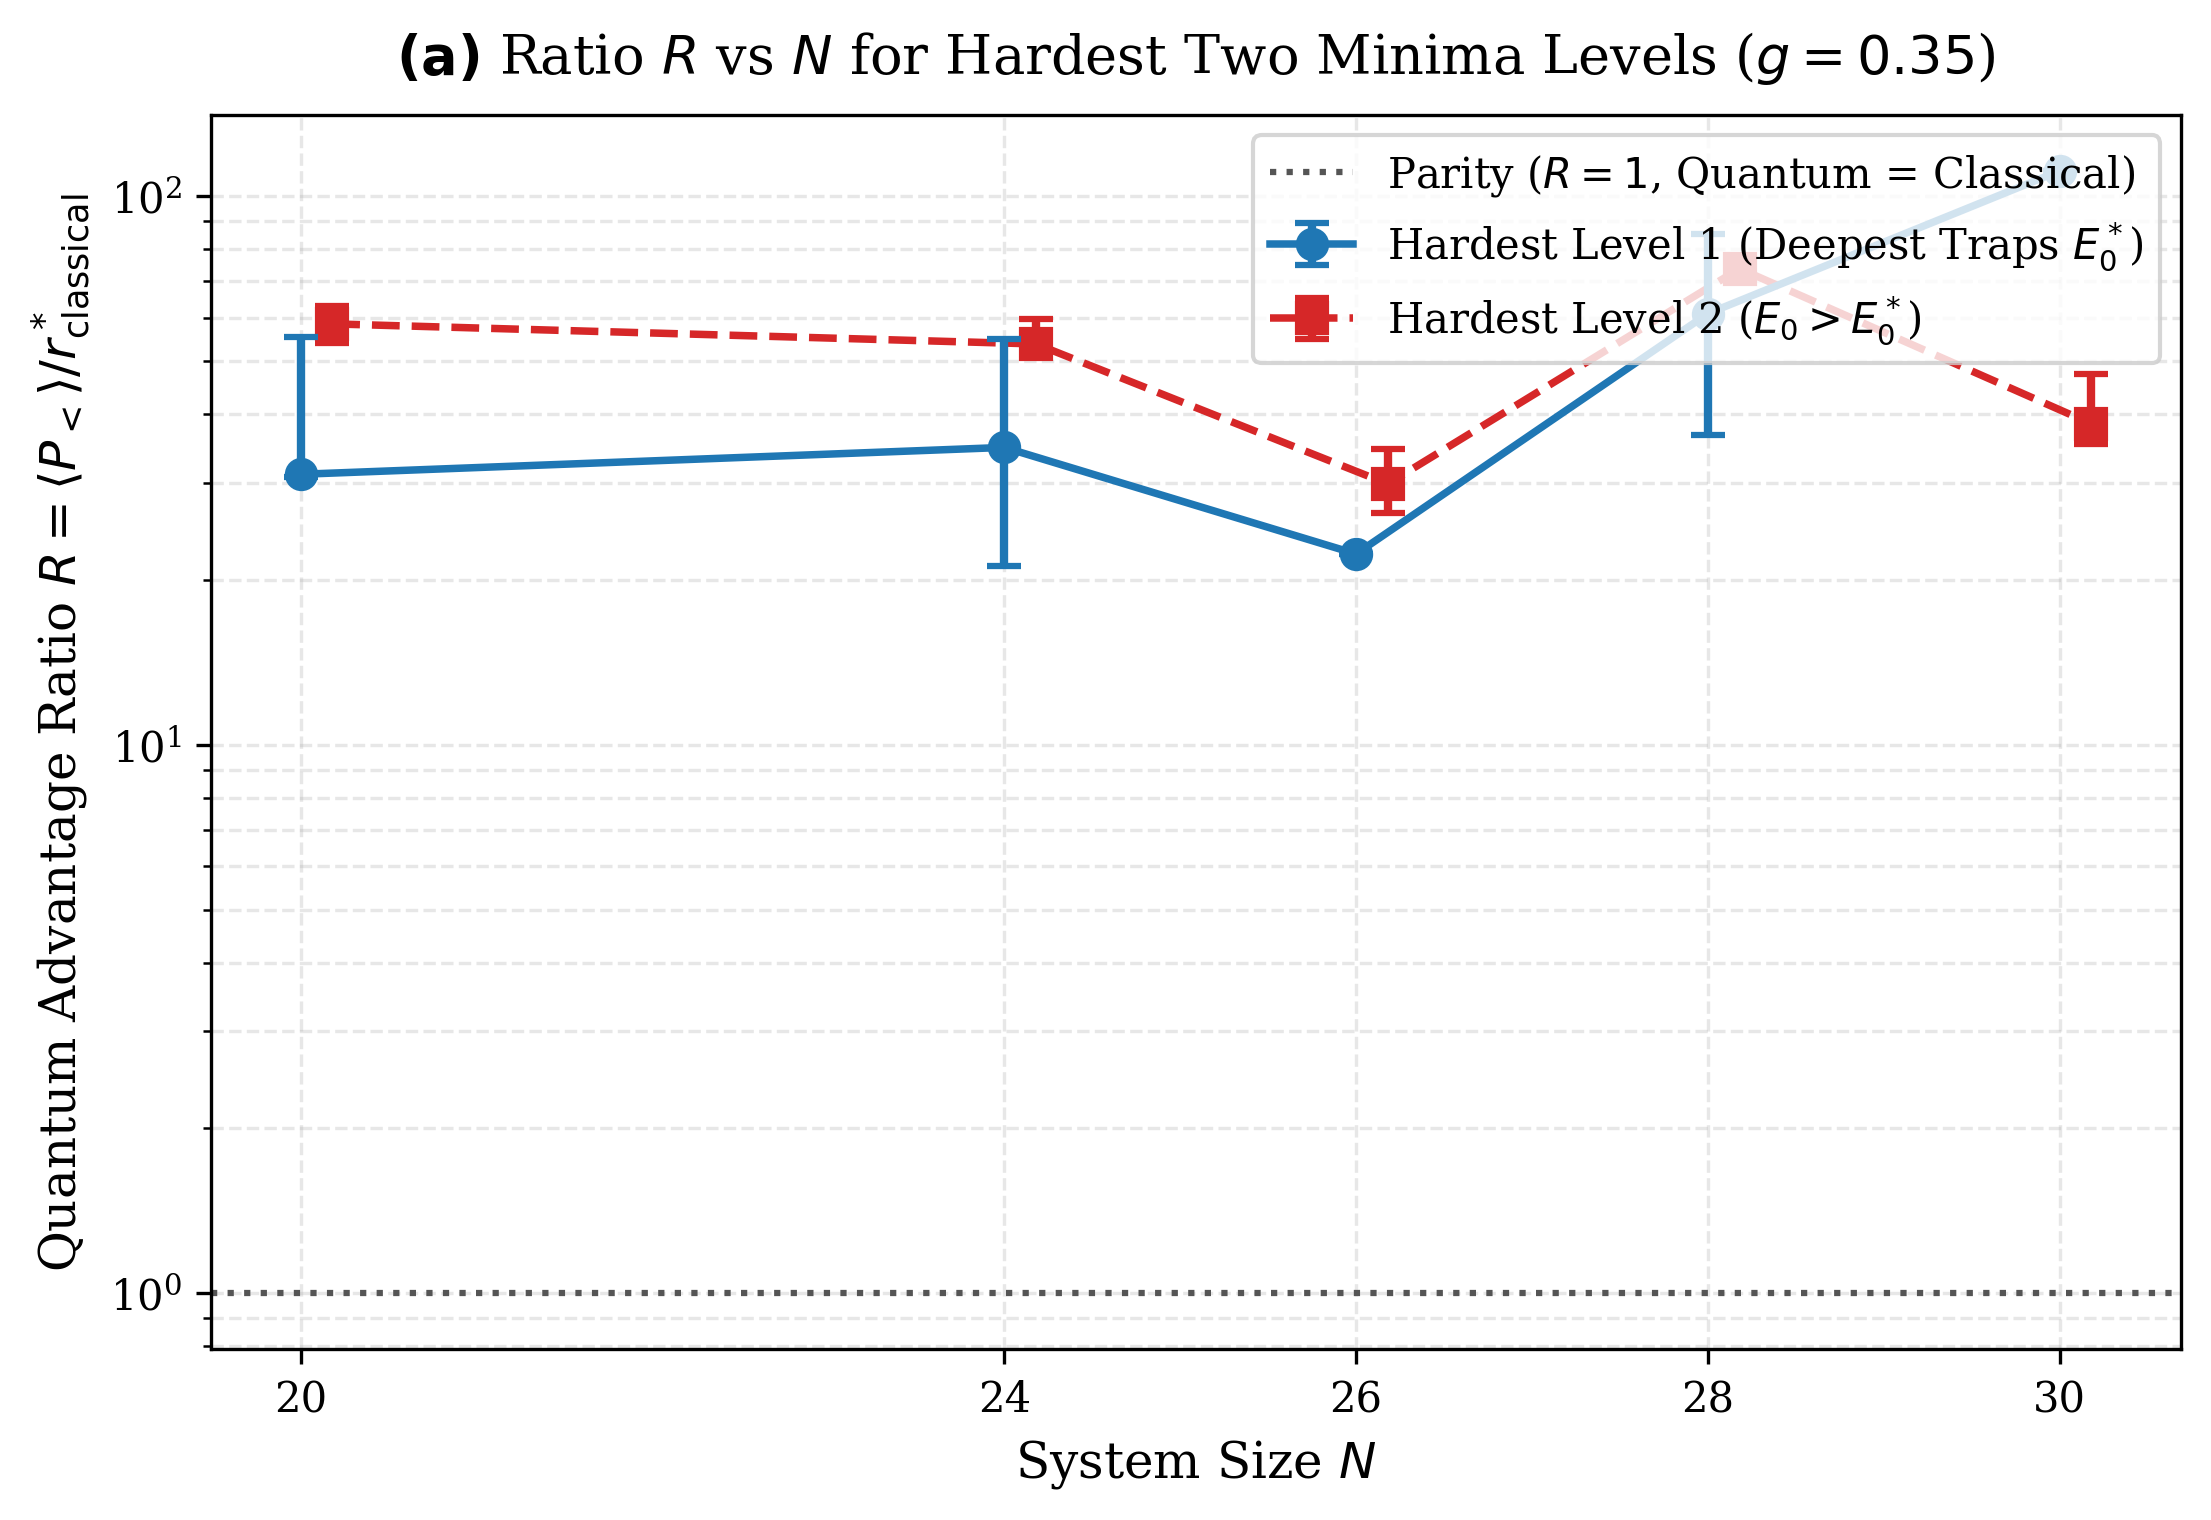
\includegraphics[width=\columnwidth]{fig_a_ratio_R_vs_N.png}
    \caption{Quantum-to-classical escape ratio $R = \langle P_< \rangle / r_{\mathrm{classical}}^*$ versus system size $N$ for Level~1 (deepest traps) and Level~2 (second-hardest traps) at $g = 0.35$. Points denote sample medians with $68\%$ bootstrap confidence intervals ($B = 2000$). The dotted line denotes parity ($R = 1$).}
    \label{fig:ratio_r}
\end{figure}

\begin{table*}[t]
\centering
\small
\caption{Quantum advantage ratio $R = \langle P_< \rangle / r_{\mathrm{classical}}^*$ at transverse field $g = 0.35$ across system sizes $N \in \{20, \dots, 30\}$, taking the upper envelope $r_{\mathrm{classical}}^* = \max(r^*(d^*), r_{\mathrm{restart}})$ over all classical multi-start baselines. Values report sample medians and $68\%$ bootstrap confidence intervals across symmetry-distinct traps for Level 1 (deepest classical traps) and Level 2 (second-hardest classical traps), corresponding directly to the level specifications in Table~\ref{tab:seed_levels}.}
\label{tab:ratio_summary}
\resizebox{\textwidth}{!}{%
\begin{tabular}{lccccc}
\toprule
\textbf{Energy Tier} & $N = 20$ & $N = 24$ & $N = 26$ & $N = 28$ & $N = 30$ \\
\midrule
\textbf{Level 1 (Deepest Traps)} & & & & & \\
Trap Energy $E_0$ & 34 & 52 & 61 & 70 & 75 \\
Distinct Orbits & 3 & 3 & 1 & 2 & 1 \\
Barrier Distance $d_{\min}$ Range & 6--8 & 6--9 & 6 & 6--9 & 9 \\
Sample Median $R$ & $\mathbf{31.11}$ & $\mathbf{34.82}$ & $\mathbf{22.26}$ & $\mathbf{61.09}$ & $\mathbf{111.24}$ \\
$68\%$ Bootstrap CI & $[30.72, 55.31]$ & $[21.20, 54.86]$ & $[22.26, 22.26]$ & $[36.75, 85.43]$ & $[111.24, 111.24]$ \\
\midrule
\textbf{Level 2 (Excited Traps)} & & & & & \\
Trap Energy $E_0$ & 38 & 56 & 69 & 74 & 91 \\
Distinct Orbits & 2 & 6 & 9 & 1 & 4 \\
Barrier Distance $d_{\min}$ Range & 5--7 & 5--6 & 2--6 & 6 & 5--7 \\
Sample Median $R$ & $\mathbf{58.50}$ & $\mathbf{53.77}$ & $\mathbf{29.88}$ & $\mathbf{73.77}$ & $\mathbf{38.45}$ \\
$68\%$ Bootstrap CI & $[54.00, 63.00]$ & $[51.14, 59.58]$ & $[26.46, 34.60]$ & $[73.77, 73.77]$ & $[35.36, 47.41]$ \\
\bottomrule
\end{tabular}%
}
\end{table*}

The data show $R > 1$ across all evaluated system sizes and both hardness strata, establishing a headline quantum advantage of $R \approx 22 - 111\times$ against the optimal classical kick heuristic for the deepest macroscopic traps (Level~1) and $R \approx 30 - 74\times$ for excited traps (Level~2):
\begin{itemize}
    \item \textbf{Level~1 (Deepest Traps):} For $N = 20$ (3 orbits, $E_0 = 34, d_{\min} \in [6, 8]$) and $N = 24$ (3 orbits, $E_0 = 52, d_{\min} \in [6, 9]$), the sample median ratio is $31.11$ ($68\%$ CI: $[30.72, 55.31]$) and $34.82$ ($68\%$ CI: $[21.20, 54.86]$), respectively. At $N = 26$ (1 orbit, $E_0 = 61, d_{\min} = 6$), the median is $22.26$ ($68\%$ CI: $[22.26, 22.26]$), while at $N = 28$ (2 orbits, $E_0 = 70, d_{\min} \in [6, 9]$) it reaches $61.09$ ($68\%$ CI: $[36.75, 85.43]$). At the largest evaluated system size ($N = 30$, 1 orbit, $E_0 = 75, d_{\min} = 9$), quantum dynamics maintain a decisive advantage of $R = 111.24$ ($68\%$ CI: $[111.24, 111.24]$) over the optimal classical perturbation baseline within the standardized evaluation window $[10.0, 38.5]$. As discussed in Section~\ref{subsec:window}, this value serves as a conservative lower bound because the wavepacket tunneling front continues to rise past $t = 38.5$.
    \item \textbf{Level~2 (Second-Hardest Traps):} Traps in the second-hardest stratum show an extensive and consistent quantum advantage across all sizes, with median ratios consistently spanning between $30\times$ and $74\times$: $R = 58.50$ ($68\%$ CI: $[54.00, 63.00]$) at $N = 20$ (2 orbits, $E_0 = 38, d_{\min} \in [5, 7]$), $R = 53.77$ ($68\%$ CI: $[51.14, 59.58]$) at $N = 24$ (6 orbits, $E_0 = 56, d_{\min} \in [5, 6]$), $R = 29.88$ ($68\%$ CI: $[26.46, 34.60]$) at $N = 26$ (9 orbits, $E_0 = 69, d_{\min} \in [2, 6]$), $R = 73.77$ ($68\%$ CI: $[73.77, 73.77]$) at $N = 28$ (1 orbit, $E_0 = 74, d_{\min} = 6$), and $R = 38.45$ ($68\%$ CI: $[35.36, 47.41]$) at $N = 30$ (4 orbits, $E_0 = 91, d_{\min} \in [5, 7]$).
\end{itemize}

This behavior reflects differing search mechanisms. Classical perturbations frequently land configurations on plateaus that re-converge into the original trap. Coherent quantum dynamics allow amplitude to penetrate barriers, populating lower-energy basins without fully traversing intermediate states.

\begin{figure*}[t]
    \centering
    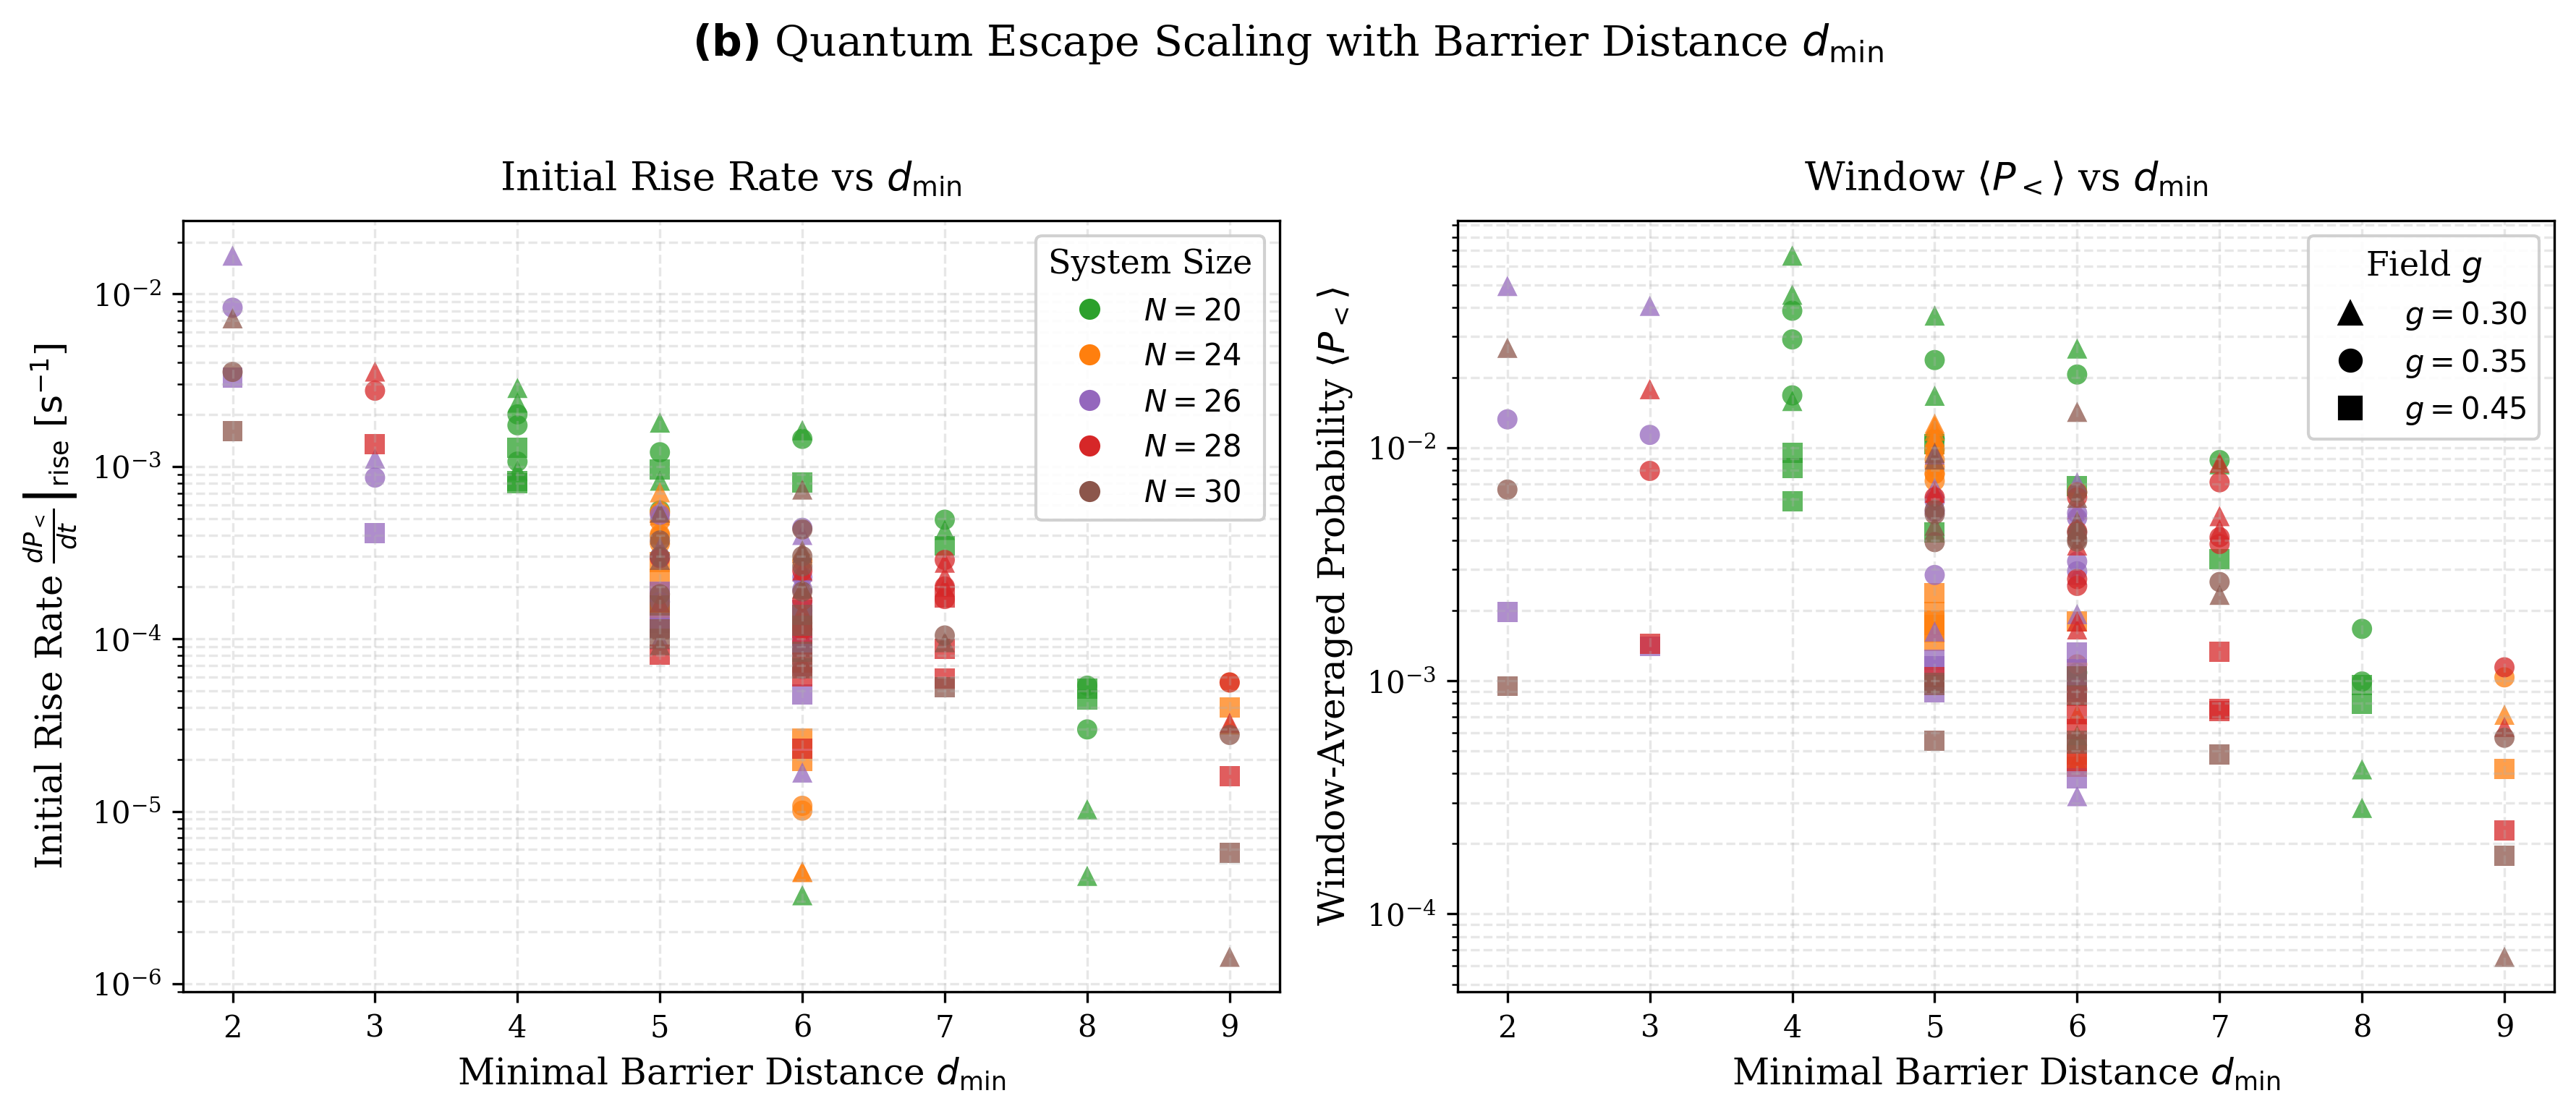
\includegraphics[width=0.92\textwidth]{fig_b_rise_rate_and_pless_vs_dmin.png}
    \caption{Dependence of quantum escape dynamics on minimal barrier distance $d_{\min}$. Left: Initial rise rate $\left.\frac{dP_<}{dt}\right|_{\mathrm{rise}}$. Right: Window-averaged escape probability $\langle P_< \rangle$. Data points are colored by system size $N \in [20, 30]$ and shaped by coupling strength $g \in \{0.30, 0.35, 0.45\}$.}
    \label{fig:rise_rate_dmin}
\end{figure*}

\begin{figure*}[t]
    \centering
    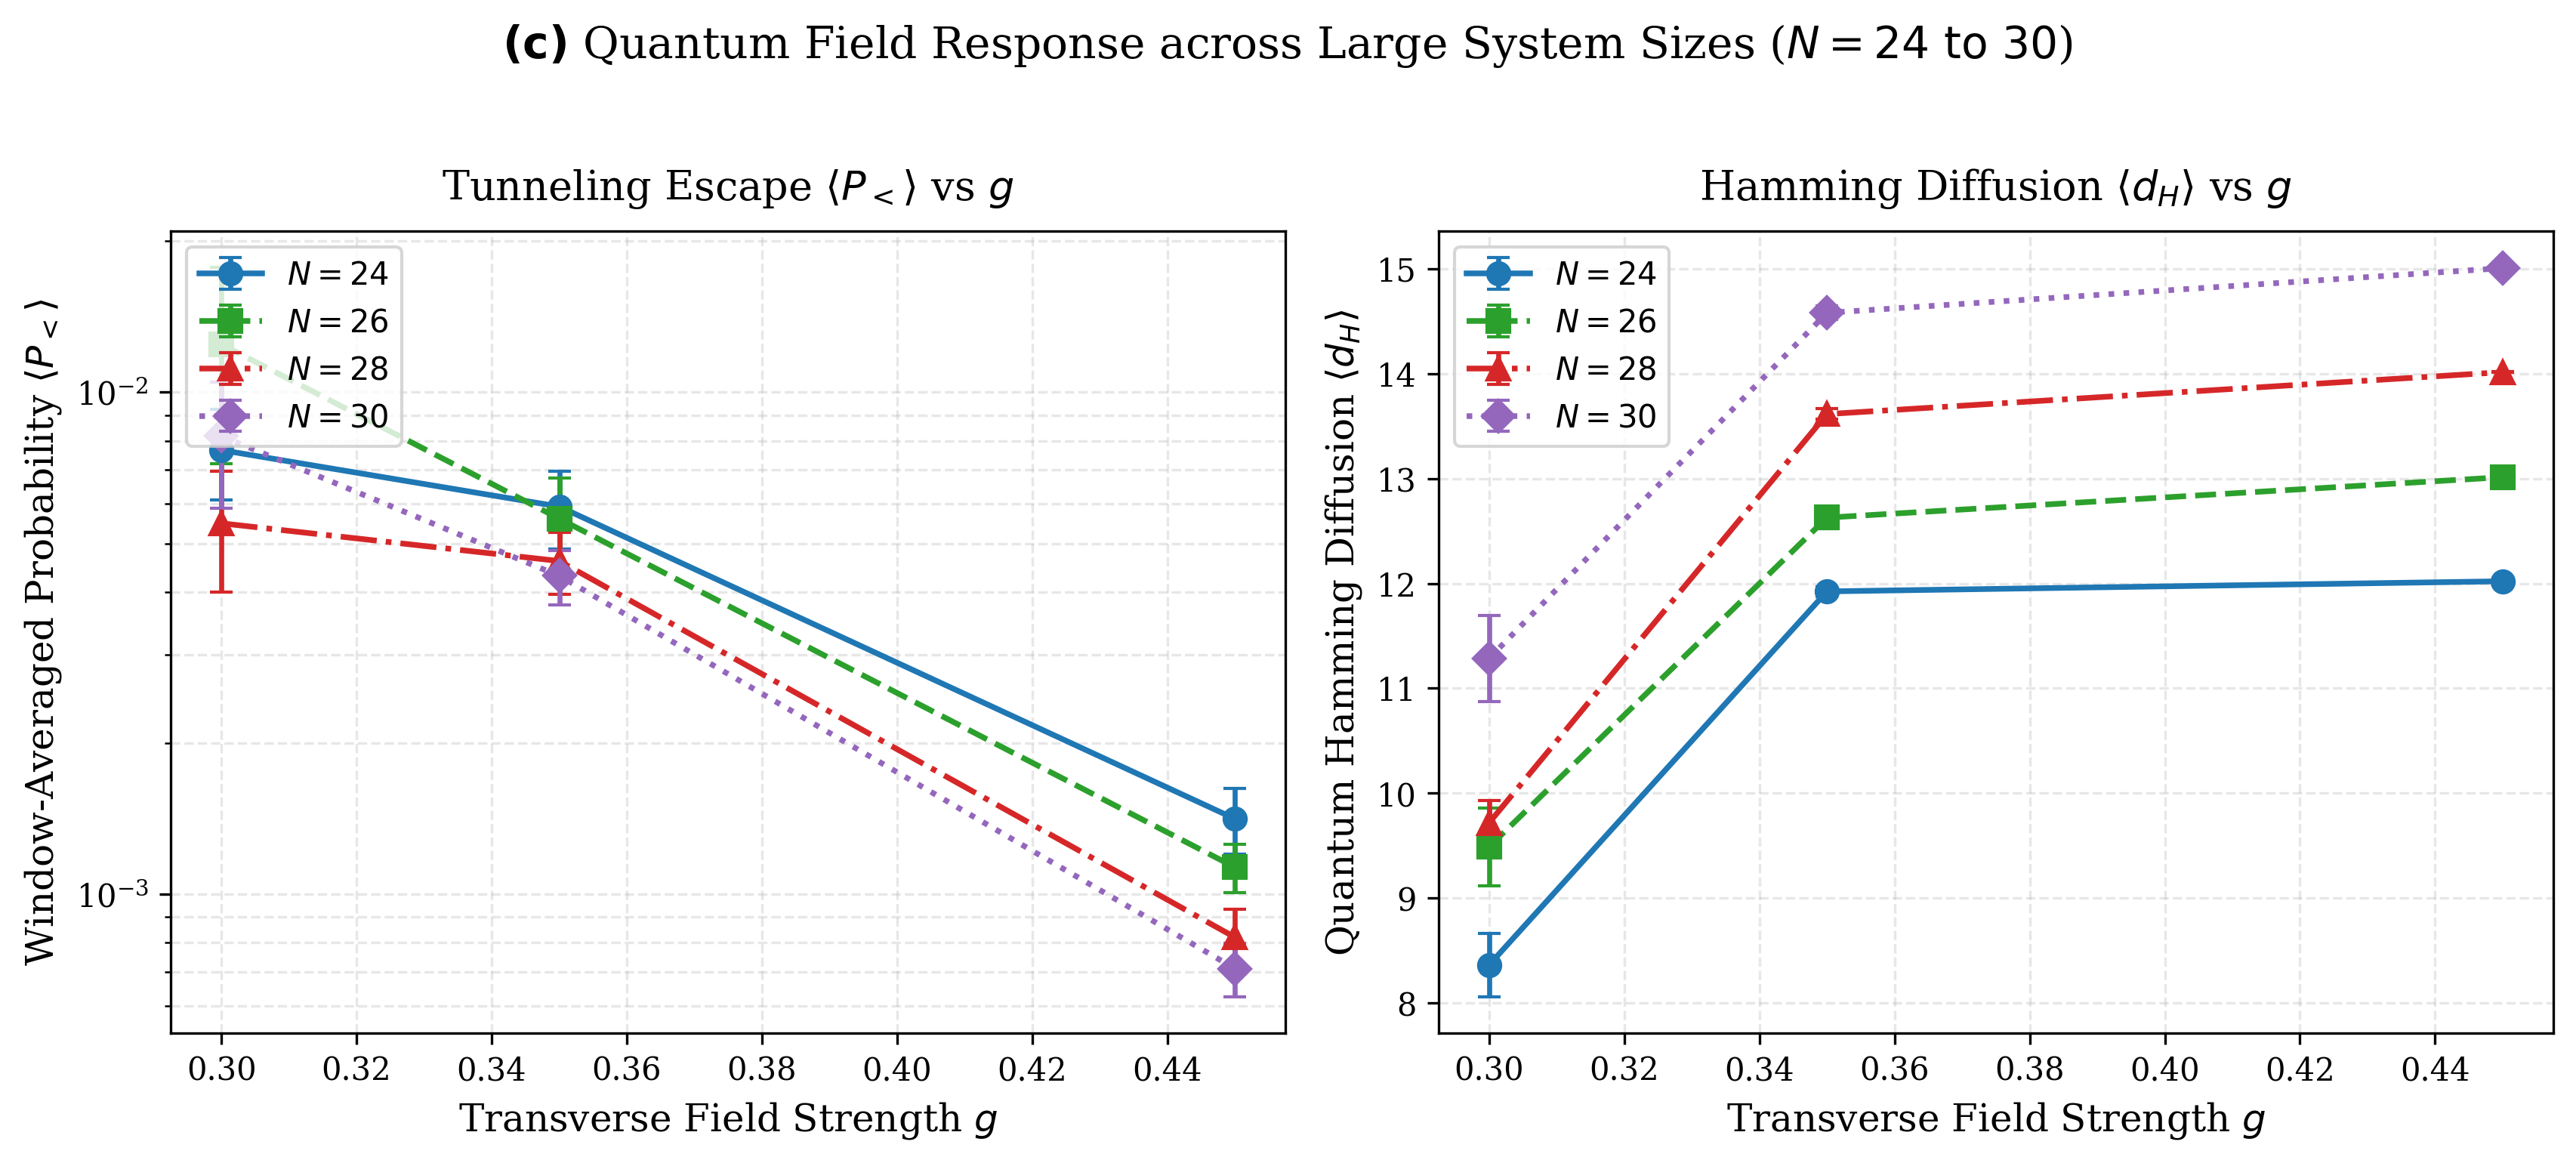
\includegraphics[width=0.88\textwidth]{fig_c_pless_and_dh_vs_g.png}
    \caption{Effect of driver strength $g$ on quantum escape and hypercube diffusion for $N \in \{24, 26, 28, 30\}$. Left: Window-averaged escape probability $\langle P_< \rangle$. Right: Mean Hamming displacement $\langle d_H \rangle$. Error bars indicate standard error of the mean (SEM).}
    \label{fig:pless_dh_g}
\end{figure*}

\subsection{Escape Dynamics across Barrier Distances and Energy Tiers}
Figure~\ref{fig:rise_rate_dmin} presents the initial rise rate $\left.\frac{dP_<}{dt}\right|_{\mathrm{rise}}$ and window-averaged escape probability $\langle P_< \rangle$ across all evaluated traps as functions of the minimal barrier distance $d_{\min} \in [2, 9]$. 

Inspection of the data reveals that minimal barrier distance $d_{\min}$ alone does not uniquely organize escape efficiency:
\begin{enumerate}
    \item \textbf{Energy Tier Stratification over Coordinate Distance:} 
    Inspection of Figure~\ref{fig:rise_rate_dmin} reveals that minimal barrier distance $d_{\min}$ alone does not uniquely predict escape probability. For a fixed barrier distance (for instance, $d_{\min} = 6$), window escape probabilities vary by nearly two orders of magnitude (ranging from $\langle P_< \rangle \approx 3.2 \times 10^{-4}$ up to $1.4 \times 10^{-2}$) depending on the trap's energy tier $E_0$. The deepest classical traps (Level~1, $E_0^*$, which feature wide barriers $d_{\min} = 6 - 9$) systematically exhibit the lowest window escape probabilities ($\langle P_< \rangle \sim 5.7 \times 10^{-4} - 1.1 \times 10^{-3}$ across $N \in [20, 30]$), while excited local minima (Level~2 and above, with $d_{\min} = 2 - 7$) achieve escape probabilities one to two orders of magnitude higher (e.g., $\langle P_< \rangle \approx 3.9 \times 10^{-3} - 1.7 \times 10^{-2}$). This separation reflects the volume of the target manifold $\mathcal{S}_< = \{s : E(s) < E_0\}$: for excited traps, $\mathcal{S}_<$ encompasses extensive lower-lying basins, whereas for Level~1 traps it is restricted to rare states near the global optimum ($P_{\mathrm{blind}} \sim 10^{-8}$ at $N = 30$).
    
    \item \textbf{Absence of Direct $d_{\min}$-th Order Perturbative Tunneling:} 
    A localized, semiclassical tunneling process along a 1D coordinate path of length $d_{\min}$ would predict transition amplitudes scaling as $(g / \Delta E)^{d_{\min}}$, implying that the initial rise rate should scale as a steep power law $g^{\alpha}$ with $\alpha \approx d_{\min}$ on log-log axes. Testing this scaling empirically yields effective exponents $\alpha = \frac{d \ln(\mathrm{rise~rate})}{d \ln g}$ that do not track $d_{\min}$: across traps with wide barriers ($d_{\min} = 9$), the median empirical slope between $g = 0.30$ and $0.35$ is $+3.63$ (and $+3.50$ across Rank~1 traps, vastly below the predicted coordinate exponent of $9$), while for $d_{\min} = 5 - 7$ the response is flat or mildly negative due to early dispersion.
    
    \item \textbf{Energy-Selective Delocalized Transfer:} 
    Coupled with the observation that Hamming diffusion expands to the hypercube bulk ($\langle d_H \rangle \approx N/2$, see Section~\ref{subsec:field_regimes}), these results demonstrate that quantum escape does not proceed via a narrow coordinate trajectory. Instead, the transverse field induces delocalized mixing across Hamming shells, while the potential landscape $\hat{H}_B / N$ acts as a spectral filter that concentrates amplitude into lower-energy configurations. This explains why quantum dynamics retain robust escape flux ($\langle P_< \rangle \sim 10^{-3} - 10^{-2}$) even across wide barriers ($d_{\min} = 6 - 9$), precisely where classical perturbations degrade under the combinatorial explosion $\binom{N}{d_{\min}} \approx 10^7$.
\end{enumerate}

\subsection{Transverse-Field Regimes and Quantum Diffusion}
\label{subsec:field_regimes}
The coupling strength $g$ controls the competition between the diagonal Bernasconi potential $\hat{H}_B / N$ and the non-commuting transverse kinetic driver $\sum_i \hat{X}_i$. Figure~\ref{fig:pless_dh_g} displays the window-averaged escape probability $\langle P_< \rangle$ and mean Hamming displacement $\langle d_H \rangle = \sum_s |c_s|^2 d_H(s, s_0)$ across $g \in \{0.30, 0.35, 0.45\}$ for system sizes $N \in \{24, 26, 28, 30\}$.

A quantitative inspection of the spatial diffusion reveals three distinct physical regimes:
\begin{itemize}
    \item \textbf{Sub-Diffusive Confinement ($g = 0.30$):} At $g = 0.30$, wavepacket spreading remains strictly bounded at $\langle d_H \rangle \approx 8.36 - 11.28$, corresponding to only $69\% - 75\%$ of the hypercube midpoint $N/2$ across system sizes $N \in [24, 30]$ (e.g., $\langle d_H \rangle = 11.28 \pm 0.43$ for $N = 30$, where $N/2 = 15$; at $N = 20$, $\langle d_H \rangle = 7.90$, or $79\%$ of $N/2$). In this regime, the deep potential wells of $\hat{H}_B$ strongly confine the wavepacket. While this preserves phase coherence over extended horizons (yielding higher asymptotic escape at late times, as detailed in Section~\ref{subsec:coupling_crossover}), initial barrier penetration is slow.
    \item \textbf{Hypercube Delocalization ($g = 0.35$):} As the field increases to $g = 0.35$, spatial diffusion undergoes a pronounced expansion, with $\langle d_H \rangle$ jumping to $11.92 - 14.58$ across $N \in [24, 30]$ ($97\% - 99\%$ of $N/2$, reaching $14.58 \pm 0.06$ at $N = 30$). The wavepacket is no longer confined within the initial trap basin, achieving full delocalization across the hypercube while maintaining elevated escape probabilities ($\langle P_< \rangle \approx 4.31 \times 10^{-3} - 5.92 \times 10^{-3}$).
    \item \textbf{Ergodic Dispersion ($g \ge 0.45$):} At $g = 0.45$, Hamming displacement converges directly to the unconstrained ergodic limit $\langle d_H \rangle = N/2$ across all system sizes ($12.02$ at $N=24$, $13.01$ at $N=26$, $14.01$ at $N=28$, and $15.01$ at $N = 30$). Concurrently, the escape probability drops precipitously by nearly an order of magnitude (falling to $\langle P_< \rangle \approx 7.11 \times 10^{-4}$ at $N = 30$). Strong transverse driving completely overwhelms the classical potential, scrambling amplitude uniformly across the exponentially dominant high-energy bulk rather than channeling it into lower-energy configurations.
\end{itemize}

\paragraph{The Sharp Delocalization Edge as the Operating Optimum.}
The transition between bounded confinement at $g = 0.30$ ($\langle d_H \rangle / (N/2) \approx 70\%$) and extensive spreading at $g = 0.35$ ($\langle d_H \rangle / (N/2) > 95\%$) identifies a sharp delocalization edge between $g \approx 0.25$ and $0.35$. This represents the primary physical mechanism governing quantum escape in the Bernasconi model:
\begin{quote}
    \textit{The optimal operating regime for quantum barrier traversal sits immediately past the delocalization edge ($g \approx 0.35$).}
\end{quote}
Below this edge, the state is dynamically trapped within local potential valleys; far above it, strong kinetic fluctuations destroy energetic selectivity through unguided ergodic mixing. Operating just past the delocalization threshold provides the necessary transverse kinetic energy to overcome classical basin trapping, while preserving the spectral filtering of the Bernasconi potential $\hat{H}_B / N$ to constructively focus probability amplitude into lower-energy configurations.

\subsection{Continuous-Time Dynamics of Hard Traps}
Figure~\ref{fig:hardest_dynamics} displays the continuous trajectory $P_<(t)$ for the hardest local minimum (Rank 1 in Level 1) at each system size $N \in \{20, 24, 26, 28, 30\}$ at $g = 0.35$.

\begin{figure}[t]
    \centering
    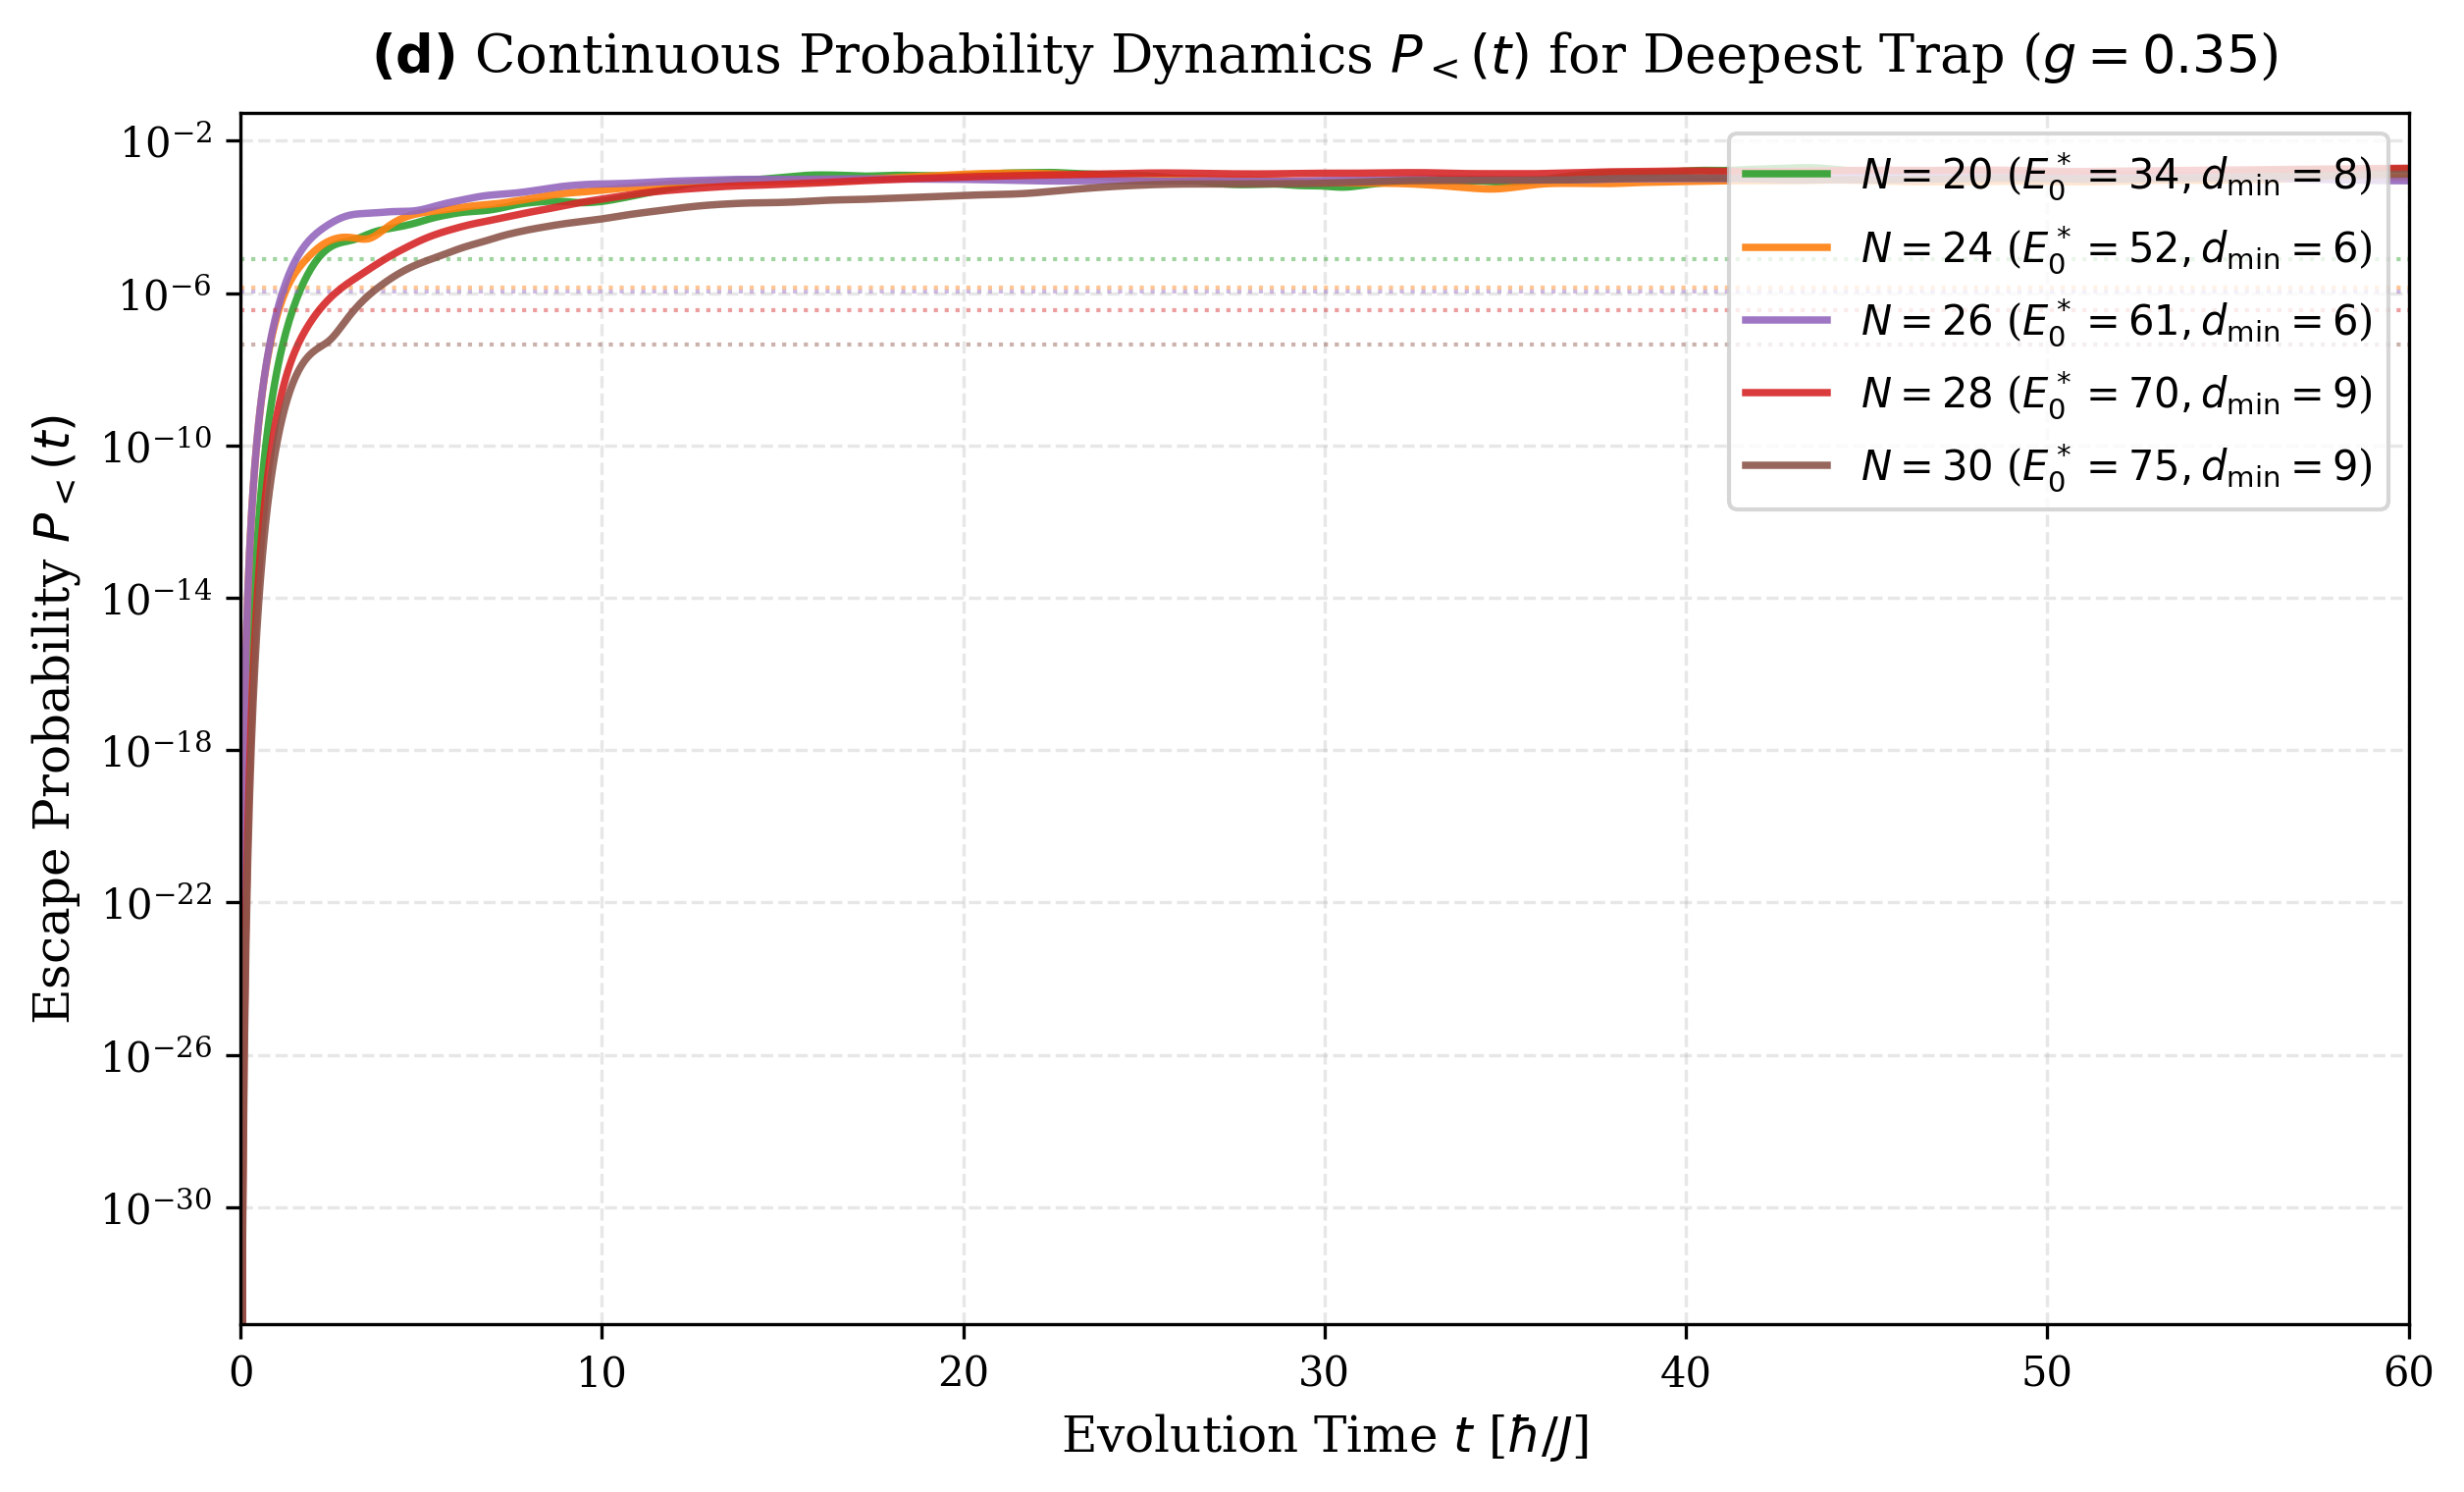
\includegraphics[width=\columnwidth]{fig_d_hardest_seed_dynamics_across_N.png}
    \caption{Continuous-time escape probability $P_<(t)$ for the hardest local minimum at each system size $N \in \{20, 24, 26, 28, 30\}$ at $g = 0.35$. Horizontal dashed lines indicate blind search probability $P_{\mathrm{blind}}$.}
    \label{fig:hardest_dynamics}
\end{figure}

Inspection of the continuous trajectories reveals two distinct dynamical regimes across time:
(i) an initial \textbf{tunneling latency phase} ($t \lesssim 3 - 5$), where multi-spin transverse mixer rotations must act iteratively to span the multi-spin ($d_{\min} \ge 6$) Hamming barrier, keeping early escape probabilities small ($P_<(1) \lesssim 10^{-7}$ across all $N$); and
(ii) an \textbf{extended rise phase} ($t \approx 5 - 30$), during which coherent tunneling flux surges by two to four orders of magnitude as amplitude penetrates the barrier into lower-energy basins (reaching $P_<(t) \sim 10^{-3}$).
Crucially, for the deepest macroscopic traps ($N = 28$ and $N = 30$), the dynamics do not establish a stationary plateau by $t = 30$ or even by $t = 38.5$; instead, escape probability continues to climb steadily through the end of the simulation horizon ($t = 60$), reaching global trajectory peaks of $1.89 \times 10^{-3}$ ($N = 28$) and $1.33 \times 10^{-3}$ ($N = 30$) at $t = 60$. As detailed in Section~\ref{subsec:window}, this persistent upward flux confirms that window-averaged escape metrics represent conservative lower bounds on the asymptotic quantum advantage.

To provide baseline geometric context for the sparsity of the target manifold, Table~\ref{tab:hardest_seeds} lists the blind volume fraction $P_{\mathrm{blind}} = |\{s : E(s) < E_0\}| / 2^N$ for the hardest local minimum (Seed Rank~1) at each system size $N \in [20, 30]$. While $P_{\mathrm{blind}}$ decreases steeply by more than two orders of magnitude from $7.63 \times 10^{-6}$ at $N = 20$ down to $4.47 \times 10^{-8}$ at $N = 30$, the quantum window probability $\langle P_< \rangle$ remains stably around $1.14 \times 10^{-3}$ to $5.70 \times 10^{-4}$. While this confirms that transverse-field dynamics concentrate amplitude into lower-energy regions rather than diffusing uniformly, blind random search is an unguided strawman. 

The rigorous benchmark headline is the quantum-to-classical escape ratio $R = \langle P_< \rangle / r_{\mathrm{classical}}^*$ against the upper envelope of classical multi-spin kicks and random restarts followed by local descent (Section~\ref{sec:results} and Table~\ref{tab:ratio_summary}). Rather than remaining static, empirical classical perturbation escape rates decay by nearly an order of magnitude across system sizes, dropping from $r_{\mathrm{classical}}^* = 3.19 \times 10^{-5}$ at $N = 20$ down to $5.13 \times 10^{-6}$ at $N = 30$, as Hamming barriers widen to $d_{\min} = 6 - 9$. Consequently, for the hardest Rank~1 configurations in Table~\ref{tab:hardest_seeds}, quantum dynamics deliver an order-of-magnitude advantage across all system sizes, ranging from $R = 22.3\times$ up to $111.2\times$ within the conservative $[10.0, 38.5]$ evaluation window.

\begin{table}[t]
    \centering
    \small
    \caption{Dynamical parameters and escape efficiency for the hardest evaluated local minimum (Rank 1) at each system size ($g = 0.35$). Seed Rank corresponds to the rank in the classical seed repository. Blind volume fraction $P_{\mathrm{blind}}$ provides landscape sparsity context, $d^*$ is the optimal classical perturbation distance, $r_{\mathrm{classical}}^* = \max(r^*(d^*), r_{\mathrm{restart}})$ is the optimal classical escape rate per evaluation, and $R = \langle P_< \rangle / r_{\mathrm{classical}}^*$ is the quantum advantage ratio. ($^{\dagger}$At $N=28$, optimal kick $d^* = 10$ yielded $r^*(10) = 3.03 \times 10^{-5}$; the upper envelope $r^*_{\mathrm{classical}} = 3.11 \times 10^{-5}$ is set by Random Restart.)}
    \label{tab:hardest_seeds}
    \resizebox{\columnwidth}{!}{%
    \begin{tabular}{ccccccccc}
        \toprule
        $N$ & Seed Rank & $E_0$ & $d_{\min}$ & $P_{\mathrm{blind}}$ & Window $\langle P_< \rangle$ & $d^*$ & $r_{\mathrm{classical}}^*$ & Ratio $R$ \\
        \midrule
        20 & 1 & 34 & 8 & $7.63 \times 10^{-6}$ & $9.93 \times 10^{-4}$ & 8  & $3.19 \times 10^{-5}$ & $\mathbf{31.1\times}$ \\
        24 & 1 & 52 & 6 & $1.43 \times 10^{-6}$ & $9.08 \times 10^{-4}$ & 4  & $2.61 \times 10^{-5}$ & $\mathbf{34.8\times}$ \\
        26 & 1 & 61 & 6 & $1.07 \times 10^{-6}$ & $9.26 \times 10^{-4}$ & 12 & $4.16 \times 10^{-5}$ & $\mathbf{22.3\times}$ \\
        28 & 1 & 70 & 9 & $3.58 \times 10^{-7}$ & $1.14 \times 10^{-3}$ & $10^{\dagger}$ & $3.11 \times 10^{-5}$ & $\mathbf{36.7\times}$ \\
        30 & 1 & 75 & 9 & $4.47 \times 10^{-8}$ & $5.70 \times 10^{-4}$ & 10 & $5.13 \times 10^{-6}$ & $\mathbf{111.2\times}$ \\
        \bottomrule
    \end{tabular}%
    }
\end{table}

\subsection{Coupling Crossover Dynamics}
\label{subsec:coupling_crossover}
Analysis of time trajectories shows that the optimal transverse-field strength $g^*$ depends on the observation horizon. While $g = 0.35$ provides faster tunneling at early times, $g = 0.30$ exhibits slower initial growth but preserves phase coherence longer, matching or exceeding $g = 0.35$ at later times for deep traps.

\begin{table}[t]
\centering
\small
\caption{Escape probability $P_<(t)$ comparing couplings $g = 0.30$ and $g = 0.35$ for deep evaluated traps ($N = 24$ Rank~1, $N = 28$ Rank~2, $N = 30$ Rank~2). Early on ($t \le 10$), $g = 0.35$ leads. Later ($t \ge 45 - 50$), $g = 0.30$ preserves coherence in the low-energy manifold, closing the gap or surpassing $g = 0.35$.}
\label{tab:coupling_crossover}
\resizebox{\columnwidth}{!}{%
\begin{tabular}{lccccc}
\toprule
$N$ & Time $t$ & $P_<(0.30)$ & $P_<(0.35)$ & $\frac{P_<(0.30)}{P_<(0.35)}$ & Dynamic Regime \\
\midrule
\textbf{$N = 24$ (Rank 1)} & $5.0$ & $5.11 \times 10^{-5}$ & $1.27 \times 10^{-4}$ & $0.40$ & $g = 0.35$ faster rise \\
& $10.0$ & $1.25 \times 10^{-4}$ & $5.04 \times 10^{-4}$ & $0.25$ & $g = 0.35$ leads \\
& $38.5$ & $5.83 \times 10^{-4}$ & $7.88 \times 10^{-4}$ & $0.74$ & $g = 0.30$ catching up \\
& $50.0$ & $8.96 \times 10^{-4}$ & $8.49 \times 10^{-4}$ & $\mathbf{1.06}$ & \textbf{Crossover} \\
& $55.0$ & $1.02 \times 10^{-3}$ & $9.43 \times 10^{-4}$ & $\mathbf{1.08}$ & $g = 0.30$ superior \\
\midrule
\textbf{$N = 28$ (Rank 2)} & $10.0$ & $1.92 \times 10^{-4}$ & $5.66 \times 10^{-4}$ & $0.34$ & $g = 0.35$ leads \\
& $38.5$ & $4.02 \times 10^{-3}$ & $4.76 \times 10^{-3}$ & $0.84$ & $g = 0.30$ catching up \\
& $60.0$ & $8.85 \times 10^{-3}$ & $7.82 \times 10^{-3}$ & $\mathbf{1.13}$ & \textbf{Crossover} \\
\midrule
\textbf{$N = 30$ (Rank 2)} & $10.0$ & $8.64 \times 10^{-4}$ & $1.52 \times 10^{-3}$ & $0.57$ & $g = 0.35$ leads \\
& $38.5$ & $9.43 \times 10^{-3}$ & $4.93 \times 10^{-3}$ & $\mathbf{1.91}$ & $g = 0.30$ overtakes \\
& $60.0$ & $1.23 \times 10^{-2}$ & $5.34 \times 10^{-3}$ & $\mathbf{2.31}$ & \textbf{$g = 0.30$ leads} \\
\bottomrule
\end{tabular}%
}
\end{table}

This crossover, shown in Table~\ref{tab:coupling_crossover}, reflects a trade-off:
(i) \textit{Early driving ($g = 0.35$)} increases the tunneling matrix element $\sim (g/\Delta E)^{d_{\min}}$, driving a faster initial rise $dP_</dt$;
(ii) \textit{Late dispersion} under stronger coupling accelerates diffusion toward the hypercube bulk ($\langle d_H \rangle \to N/2$); and
(iii) \textit{Late coherence ($g = 0.30$)} maintains amplitude concentration in low-Hamming-distance shells longer, surpassing $g = 0.35$ by $t \approx 50 - 60$.

\subsection{Evaluation Window Truncation and Lower Bounds}
\label{subsec:window}
Continuous trajectory records indicate that for deep traps, escape probability $P_<(t)$ is still rising at the end of the simulation horizon ($t = 60$). Evaluating performance over a fixed measurement window $[10.0, 38.5]$ therefore truncates the late-time increase, producing a conservative lower bound on asymptotic advantage.

\begin{table}[t]
\centering
\small
\caption{Comparison of window-averaged escape probability $\langle P_< \rangle_{[10, 38.5]}$ versus late-time escape probability $P_<(t = 60)$ for deep traps across $N \in \{24, 28, 30\}$.}
\label{tab:window_underestimation}
\resizebox{\columnwidth}{!}{%
\begin{tabular}{lcccccc}
\toprule
$N$ & Rank & $E_0$ & $d_{\min}$ & Field $g$ & $\langle P_< \rangle_{[10, 38.5]}$ & $P_<(t = 60)$ \\
\midrule
24 & Rank 1 & 52 & 6 & 0.30 & $4.52 \times 10^{-4}$ & $8.19 \times 10^{-4}$ ($1.81\times$) \\
24 & Rank 3 & 52 & 6 & 0.30 & $7.18 \times 10^{-4}$ & $1.39 \times 10^{-3}$ ($1.94\times$) \\
28 & Rank 1 & 70 & 9 & 0.35 & $1.14 \times 10^{-3}$ & $1.89 \times 10^{-3}$ ($1.65\times$) \\
28 & Rank 2 & 70 & 6 & 0.30 & $1.66 \times 10^{-3}$ & $8.85 \times 10^{-3}$ ($5.32\times$) \\
30 & Rank 1 & 75 & 9 & 0.35 & $5.70 \times 10^{-4}$ & $1.33 \times 10^{-3}$ ($2.33\times$) \\
30 & Rank 2 & 91 & 5 & 0.30 & $4.63 \times 10^{-3}$ & $1.23 \times 10^{-2}$ ($2.67\times$) \\
30 & Rank 3 & 91 & 6 & 0.30 & $4.83 \times 10^{-3}$ & $1.11 \times 10^{-2}$ ($2.30\times$) \\
\bottomrule
\end{tabular}%
}
\end{table}

As shown in Table~\ref{tab:window_underestimation}, across deep traps with $d_{\min} \ge 5$, $P_<(60)$ exceeds the window average by a factor between $1.6\times$ and $5.3\times$. For example, at $N = 30$ Rank~1 ($E_0 = 75, d_{\min} = 9$) under $g = 0.35$, $P_<(t)$ rises from $8.86 \times 10^{-5}$ at $t = 10$ to $1.03 \times 10^{-3}$ at $t = 38.5$, reaching $1.33 \times 10^{-3}$ at $t = 60$ ($2.33\times$ higher than the window average). This systematically understates the true asymptotic tunneling probability.

Importantly, this underestimation renders all advantage ratios reported in Table~\ref{tab:ratio_summary} (and Figure~\ref{fig:ratio_r}) strictly conservative lower bounds. Under the frozen headline protocol ($g = 0.35$), quantum dynamics achieve decisive advantage ($R \gg 1$) across all sizes and tiers, yielding $R = 111.24$ for the deepest Level~1 trap (Rank~1) at $N = 30$ within $[10.0, 38.5]$ and scaling to even higher values at longer horizons. 

Even under the weaker field $g = 0.30$, where slower initial rise limits early-to-intermediate tunneling flux, quantum dynamics still achieve $R = 12.8\times$ for Level~1 at $N = 30$ ($\langle P_< \rangle = 6.56 \times 10^{-5}$ vs.\ $r_{\mathrm{classical}}^* = 5.13 \times 10^{-6}$); furthermore, as demonstrated in Table~\ref{tab:coupling_crossover} for Level~2 excited traps ($N = 30$ Rank~2), $g = 0.30$ undergoes a late-time coherence crossover around $t \approx 45 - 50$, surpassing $g = 0.35$ by $t = 60$ ($P_<(60) = 1.23 \times 10^{-2}$ vs.\ $5.34 \times 10^{-3}$, a $2.31\times$ advantage). Consequently, whether evaluated at the headline field $g = 0.35$ or evolved to late times at $g = 0.30$, simulated quantum dynamics consistently outperform classical perturbation baselines across the Bernasconi landscape.

% -------------------------------------------------------------
\section{Conclusion and Outlook}
\label{sec:conclusion}
% -------------------------------------------------------------
In this work, we evaluated continuous-time transverse-field quantum dynamics as an escape mechanism from deep local minima in the Bernasconi spin model. Using GPU statevector simulations for macroscopic system sizes $N \in [20, 30]$ ($2^{20} \approx 1.05 \times 10^6$ to $2^{30} \approx 1.07 \times 10^9$ states) initialized directly in classical local traps, we established:
\begin{enumerate}
    \item \textbf{Quantum vs. Classical Escape Advantage:} Across evaluated sizes $N \in [20, 30]$ at $g = 0.35$, quantum dynamics achieve a decisive advantage over the best classical perturbation heuristics (optimal multi-spin kicks followed by local descent). For the deepest classical traps (Level~1), quantum dynamics achieve headline advantage ratios of $R \approx 22 - 111\times$ across system sizes $N = 20 - 30$ (with sample medians reaching $R = 61.09$ at $N = 28$ and $R = 111.24$ at $N = 30$), while excited (Level~2) traps exhibit median ratios consistently between $30\times$ and $74\times$.
    \item \textbf{Delocalized Transfer vs. Coordinate Barriers:} Rather than proceeding via direct $d_{\min}$-order localized tunneling with exponential distance decay, quantum escape is governed by energy-selective delocalized transfer across the hypercube ($\langle d_H \rangle \approx N/2$), where target manifold density dominates over coordinate distance $d_{\min}$. Consequently, quantum dynamics sustain robust escape flux ($\langle P_< \rangle \sim 10^{-3} - 10^{-2}$) even across wide barriers ($d_{\min} = 6 - 9$), precisely where classical perturbations degrade under the combinatorial search volume $\binom{N}{d_{\min}} \approx 10^7$.
    \item \textbf{Delocalization Edge and Dynamical Regimes:} A sharp delocalization edge separates sub-diffusive confinement at $g = 0.30$ ($\langle d_H \rangle \approx 70\%$ of $N/2$) from hypercube-wide spreading at $g = 0.35$ ($\langle d_H \rangle > 95\%$ of $N/2$). The optimal operational protocol ($g = 0.35$) sits immediately past this delocalization threshold, maximizing rapid barrier escape while retaining the spectral filtering of the Bernasconi potential before unguided ergodic dispersion sets in at $g \ge 0.45$ ($\langle d_H \rangle = N/2$). Over extended horizons ($t \ge 40$), the sub-diffusive field $g = 0.30$ avoids dephasing to sustain higher asymptotic coherence. While the blind volume fraction drops to $P_{\mathrm{blind}} = 4.47 \times 10^{-8}$ at $N = 30$, quantum dynamics maintain window escape probabilities around $10^{-3}$, sustaining non-zero flux where classical search volume expands exponentially.
\end{enumerate}

\paragraph{Limitations.}
Exact statevector simulation requires storing $2^N$ complex amplitudes, bounding single-node GPU simulation around $N = 30$ ($24-32\,\text{GB}$ active VRAM for $16\,\text{GiB}$ statevector amplitudes plus energy cache and cuStateVec workspace; $N = 32$ requires $>64\,\text{GB}$). In addition, these simulations assume unitary evolution without decoherence, whereas physical processors experience gate infidelity, $T_1$, and $T_2$ noise.

\paragraph{Outlook.}
Promising directions include evaluating randomized Hamiltonian simulation methods (such as qDRIFT~\cite{campbell2019} and SqDRIFT~\cite{piccinelli2025}) to reduce the $\mathcal{O}(N^3)$ four-body gate count on physical processors, testing time-dependent transverse-field schedules $g(t)$, investigating tensor network (MPS) approximations for $N > 30$, and feeding quantum-sampled low-energy configurations into sparse Krylov subspace diagonalization (SKQD)~\cite{yu2025}.

% -------------------------------------------------------------
% References
% -------------------------------------------------------------
\begin{thebibliography}{99}

\bibitem{bernasconi1987}
J.~Bernasconi,
``Low autocorrelation binary sequences: statistical mechanics and extreme value statistics,''
\emph{Journal de Physique}, vol.~48, no.~4, pp.~559--567, 1987.
\doi{10.1051/jphys:01987004804055900}

\bibitem{mertens1998}
S.~Mertens and C.~Bessenrodt,
``On the ground states of the {B}ernasconi model,''
\emph{Journal of Physics A: Mathematical and General}, vol.~31, no.~16, pp.~3731--3749, 1998.
\doi{10.1088/0305-4470/31/16/009}

\bibitem{packebusch2016}
T.~Packebusch and S.~Mertens,
``Low autocorrelation binary sequences to $N=105$,''
\emph{Journal of Physics A: Mathematical and Theoretical}, vol.~49, no.~16, p.~165001, 2016.
\doi{10.1088/1751-8113/49/16/165001}

\bibitem{mertens1996}
S.~Mertens,
``Exhaustive search for low-autocorrelation binary sequences,''
\emph{Journal of Physics A: Mathematical and General}, vol.~29, no.~18, pp.~L473--L481, 1996.
\doi{10.1088/0305-4470/29/18/002}

\bibitem{marinari1994}
E.~Marinari, G.~Parisi, and F.~Ritort,
``Replica field theory for deterministic models: II. A non-random spin glass with glassy behaviour,''
\emph{Journal of Physics A: Mathematical and General}, vol.~27, no.~23, pp.~7647--7668, 1994.
\doi{10.1088/0305-4470/27/23/011}

\bibitem{prestwich2007}
S.~Prestwich,
``Exploiting problem structure for low autocorrelation binary sequences,''
\emph{Annals of Operations Research}, vol.~156, no.~1, pp.~89--100, 2007.
\doi{10.1007/s10479-007-0223-9}

\bibitem{kadowaki1998}
T.~Kadowaki and H.~Nishimori,
``Quantum annealing in the transverse Ising model,''
\emph{Physical Review E}, vol.~58, no.~5, pp.~5355--5363, 1998.
\doi{10.1103/PhysRevE.58.5355}

\bibitem{farhi2001}
E.~Farhi, J.~Goldstone, S.~Gutmann, J.~Lapan, A.~Lundgren, and D.~Preda,
``A quantum adiabatic evolution algorithm applied to random instances of an NP-complete problem,''
\emph{Science}, vol.~292, no.~5516, pp.~472--475, 2001.
\doi{10.1126/science.1057726}

\bibitem{santoro2002}
G.~E.~Santoro, R.~Marto{\v{n}}{\'a}k, E.~Tosatti, and R.~Car,
``Theory of quantum annealing of an Ising spin glass,''
\emph{Science}, vol.~295, no.~5564, pp.~2427--2430, 2002.
\doi{10.1126/science.1068774}

\bibitem{denchev2016}
V.~S.~Denchev, S.~Boixo, S.~V.~Isakov, N.~Ding, R.~Babbush, V.~N.~Smelyanskiy, J.~M.~Martinis, and H.~Neven,
``What is the computational value of finite-range tunneling?''
\emph{Physical Review X}, vol.~6, no.~3, p.~031015, 2016.
\doi{10.1103/PhysRevX.6.031015}

\bibitem{trotter1959}
H.~F.~Trotter,
``On the product of semi-groups of operators,''
\emph{Proceedings of the American Mathematical Society}, vol.~10, no.~4, pp.~545--551, 1959.
\doi{10.1090/S0002-9939-1959-0108732-6}

\bibitem{suzuki1976}
M.~Suzuki,
``Generalized Trotter's formula and systematic approximants of exponential operators and inner derivations with applications to many-body problems,''
\emph{Communications in Mathematical Physics}, vol.~51, no.~2, pp.~183--190, 1976.
\doi{10.1007/BF01609348}

\bibitem{childs2021}
A.~M.~Childs, Y.~Su, M.~C.~Tran, N.~Wiebe, and S.~Zhu,
``Theory of Trotter error with commutator scaling,''
\emph{Physical Review X}, vol.~11, no.~1, p.~011020, 2021.
\doi{10.1103/PhysRevX.11.011020}

\bibitem{custatevec}
{NVIDIA Corporation},
``cuQuantum SDK: cuStateVec High Performance State Vector Library,''
\url{https://developer.nvidia.com/cuquantum-sdk}, 2023.

\bibitem{marti2003}
R.~Mart{\'i},
``Multi-start methods,''
in \emph{Handbook of Metaheuristics}, ser. International Series in Operations Research \& Management Science, vol.~57, pp.~355--368, Springer, Boston, MA, 2003.
\doi{10.1007/0-306-48056-5_12}

\bibitem{efron1994}
B.~Efron and R.~J.~Tibshirani,
\emph{An Introduction to the Bootstrap},
ser. Monographs on Statistics and Applied Probability, vol.~57. CRC Press / Chapman \& Hall, 1994.

\bibitem{yu2025}
J.~Yu, J.~Robledo Moreno, and others,
``Quantum-Centric Algorithm for Sample-Based Krylov Diagonalization,''
\emph{arXiv preprint arXiv:2501.09702}, 2025.

\bibitem{campbell2019}
E.~Campbell,
``A random compiler for fast Hamiltonian simulation,''
\emph{Physical Review Letters}, vol.~123, no.~7, p.~070503, 2019.
\doi{10.1103/PhysRevLett.123.070503}

\bibitem{piccinelli2025}
S.~Piccinelli and others,
``Quantum chemistry with provable convergence via randomized sample-based quantum diagonalization,''
\emph{arXiv preprint arXiv:2508.02578}, 2025.

\end{thebibliography}

\end{document}
